\documentclass[11pt, a4paper]{article}
\usepackage[utf8]{inputenc}
\usepackage{listings}
\usepackage[margin=1.0in]{geometry}
\usepackage{color}
\usepackage{graphicx}
\usepackage{tabularx}
\usepackage{url}
\usepackage{float}
\usepackage{enumitem}
\usepackage{subcaption}

\lstnewenvironment{python}[1][]
{\lstset{
		language=python,
		numbers=left,
		numberstyle=\tiny,
		keywordstyle=\color{blue},       	% keyword style
		basicstyle=\footnotesize\ttfamily,	% font
		numbers=left,						% line numbers
		tabsize=2,							% tabsize in spaces
		#1}}
{}

\lstnewenvironment{bash}[1][]
{\lstset{
		language=bash,
		numbers=left,
		numberstyle=\tiny,
		numbers=none,
		basicstyle=\footnotesize\ttfamily,	% font
		tabsize=2,							% tabsize in spaces
		#1}}
{}

\lstnewenvironment{code}[1][]
{\lstset{numbers=left,
		numberstyle=\tiny,
		keywordstyle=\color{blue},       % keyword style
		basicstyle=\footnotesize\ttfamily,	% font
		numbers=left,						% line numbers
		tabsize=2,							% tabsize in spaces
		#1}}
{}

\title{DezSys06 - Verschlüsselung}
\author{Elias Frantar, Gary Ye (5AHITT)}
\date{\today{}, Wien}
\begin{document}

\lstset{
  backgroundcolor=\color{white},   % choose the background color; you must add \usepackage{color} or \usepackage{xcolor}
  basicstyle=\footnotesize,        % the size of the fonts that are used for the code
  breakatwhitespace=false,         % sets if automatic breaks should only happen at whitespace
  breaklines=true,                 % sets automatic line breaking
  captionpos=b,                    % sets the caption-position to bottom
% commentstyle=\color{mygreen},    % comment style
  deletekeywords={...},            % if you want to delete keywords from the given language
  escapeinside={\%*}{*)},          % if you want to add LaTeX within your code
  extendedchars=true,              % lets you use non-ASCII characters; for 8-bits encodings only, does not work with UTF-8
% frame=single,                    % adds a frame around the code
  keepspaces=true,                 % keeps spaces in text, useful for keeping indentation of code (possibly needs columns=flexible)
  keywordstyle=\color{blue},       % keyword style
% language=bash,                   % the language of the code
  morekeywords={*,...},            % if you want to add more keywords to the set
  numbers=none,                    % where to put the line-numbers; possible values are (none, left, right)
  numbersep=5pt,                   % how far the line-numbers are from the code
%  numberstyle=\tiny\color{gray}, % the style that is used for the line-numbers
  rulecolor=\color{black},         % if not set, the frame-color may be changed on line-breaks within not-black text (e.g. comments (green here))
  showspaces=false,                % show spaces everywhere adding particular underscores; it overrides 'showstringspaces'
  showstringspaces=false,          % underline spaces within strings only
  showtabs=false,                  % show tabs within strings adding particular underscores
%  stepnumber=1,                    % the step between two line-numbers. If it's 1, each line will be numbered
  stringstyle=\color{red},     % string literal style
  tabsize=2,                       % sets default tabsize to 2 spaces
  title=\lstname,                   % show the filename of files included with \lstinputlisting; also try caption instead of title
  belowskip=-3em,    
}

% \setlength\parindent{0pt}

\maketitle
\newpage
\tableofcontents
\newpage

\section{Requirements}

Das neu eröffnete Unternehmen iKnow Systems ist spezialisiert auf
Knowledgemanagement und bietet seinen Kunden die Möglichkeiten Daten und
Informationen jeglicher Art in eine Wissensbasis einzupflegen und anschließend
in der zentralen Wissensbasis nach Informationen zu suchen (ähnlich wikipedia).

Folgendes ist im Rahmen der Aufgabenstellung verlangt:

Entwerfen Sie ein Datenmodell, um die Eintraege der Wissensbasis zu speichern
und um ein optimitiertes Suchen von Eintraegen zu gewaehrleisten. [2Pkt]

Entwickeln Sie mittels RESTful Webservices eine Schnittstelle, um die
Wissensbasis zu verwalten. Es muessen folgende Operationen angeboten werden: -
Hinzufuegen eines neuen Eintrags - Aendern eines bestehenden Eintrags -
Loeschen eines bestehenden Eintrags

Alle Operationen muessen ein Ergebnis der Operation zurueckliefern. [3Pkt]

Entwickeln Sie in Java ein SOA Webservice, dass die Funktionalitaet Suchen
anbietet und das SOAP Protokoll einbindet. Erzeugen Sie fuer dieses Webservice
auch eine WSDL-Datei. [3Pkt]

Entwerfen Sie eine Weboberflaeche, um die RESTful Webservices zu verwenden.
[3Pkt]

Implementieren Sie einen einfachen Client mit einem User Interface (auch
Commandline UI moeglich), der das SOA Webservice aufruft. [2Pkt]

Dokumentieren Sie im weiteren Verlauf den Datentransfer mit SOAP. [1Pkt]

Protokoll ist erforderlich! [2Pkt] Info: Gruppengroesse: 2 Mitglieder Punkte:
16

Zum Testen bereiten Sie eine Routine vor, um die Wissensbasis mit einer 1
Million Datensaetze zu fuellen. Die Datensaetze sollen mindestens eine Laenge
beim Suchbegriff von 10 Zeichen und bei der Beschreibung von 100 Zeichen haben!
Ist die Performance bei der Suche noch gegeben?

Links:

JEE Webservices: http://docs.oracle.com/javaee/6/tutorial/doc/gijti.html

Apache Web Services Project: http://ws.apache.org/

Apache Axis/Axis2: http://axis.apache.org http://axis.apache.org/axis2/java/core/

IBM Article: Java Web services - JAXB and JAX-WS in Axis2:
http://www.ibm.com/developerworks/java/library/j-jws8/index.html

\section{Application Design}

The design was carefully designed such that efficiency and reliability could be
guaranteed. The UML class diagram that is shown in the following figure (see
Figure \ref{fig:uml}) represents the model classes that store the underlying
data of the backend. 

% todo: insert uml diagram

\section{Implementation}

\subsection{REST Webservice}

The REST Webservice was fully implemented within Python and using the Flask API,
especially using the Flask RESTful module. Below, we will show the esssential
part that was necessary for implementing a fully responsible RESTful API.  

The Webservice follows the design that was thoroughly described in section
\ref{sec:design}.

\subsubsection{URI}

The URI which can be used to call the different methods offered by the
webservice are listed down in the following table (Table \ref{tab:uri}).

\begin{table}[htbp]
  \centering
  \begin{tabular}{| c | c | c | l | } \hline
    \textbf{URI} & \textbf{Parameters} & \textbf{Method} & \textbf{Meaning} \\ \hline
    \lstinline|/q| & \lstinline|?tags=tag1,tag2| & \lstinline|GET| & Queries the data with the specified tags.  \\ \hline
    \lstinline|/knowledge| & \lstinline|content=str, tags=str| & \lstinline|POST| & Adds a new entry. \\ \hline
    \lstinline|/knowledge/<id>| &  & \lstinline|GET| & Retrieves the data of the given id  \\ \hline
    \lstinline|/knowledge/<id>| & \lstinline|content=str, tags=str| & \lstinline|PUT| & Updates the entry.   \\ \hline
    \lstinline|/knowledge/<id>| &  & \lstinline|DELETE| & Removes the entry with the given id \\ \hline
  \end{tabular}
  \caption{The URI options for the user}
  \label{tab:uri}
\end{table}

\subsubsection{Flask}

Two vital objects have to instantiated intially: 

\begin{lstlisting}
from flask import Flask
from flask.ext.restful import Api

app = Flask(__name__)
api = Api(app)
\end{lstlisting}
\vspace{10pt}

Now we need to define an API class for each resource that the webservice should
offer. These classes are required to implement the methods that are available,
e.g., GET, POST, PUT, ..., as Python methods with the same corresponding name,
however, in lowercase, e.g, get, put, post, etc. One example will be shown
below. 

\begin{lstlisting}
class KnowledgeAPI(Resource):
    def __init__(self):
        self.reqparse = reqparse.RequestParser()
        self.reqparse.add_argument('content', type=str)
        self.reqparse.add_argument('tags', type=str)

    def get(self, id):
        knowledge = Knowledge.query.filter_by(id=id).first()
        if knowledge is None:
            return {}
        return knowledge.mapped()

    def put(self, id):
        args = self.reqparse.parse_args()
        knowledge = Knowledge.query.filter_by(id=id).first()
        knowledge.content = args['content']
        knowledge.tags = [Tag(tag) for tag in args['tags'].split(',')]
        db.session.commit()
        return {'msg': 'Success'}

    def delete(self, id):
        knowledge = Knowledge.query.filter_by(id=id).first()
        db.session.delete(knowledge)
        db.session.commit()
        return {'msg': 'Success'}
\end{lstlisting}

\vspace{10pt}

The code is responsible for accessing the database with the elementary CRUD
commands. 

However, these classes must be added to the \lstinline|api| object first. 

\begin{lstlisting}
api.add_resource(KnowledgeQueryAPI, '/q')
\end{lstlisting}

\subsection{}

\section{Testing}

Tests with small a dataset were performed. 

\subsection{Creating the Schema}

\begin{figure}[h!]
  \centering
  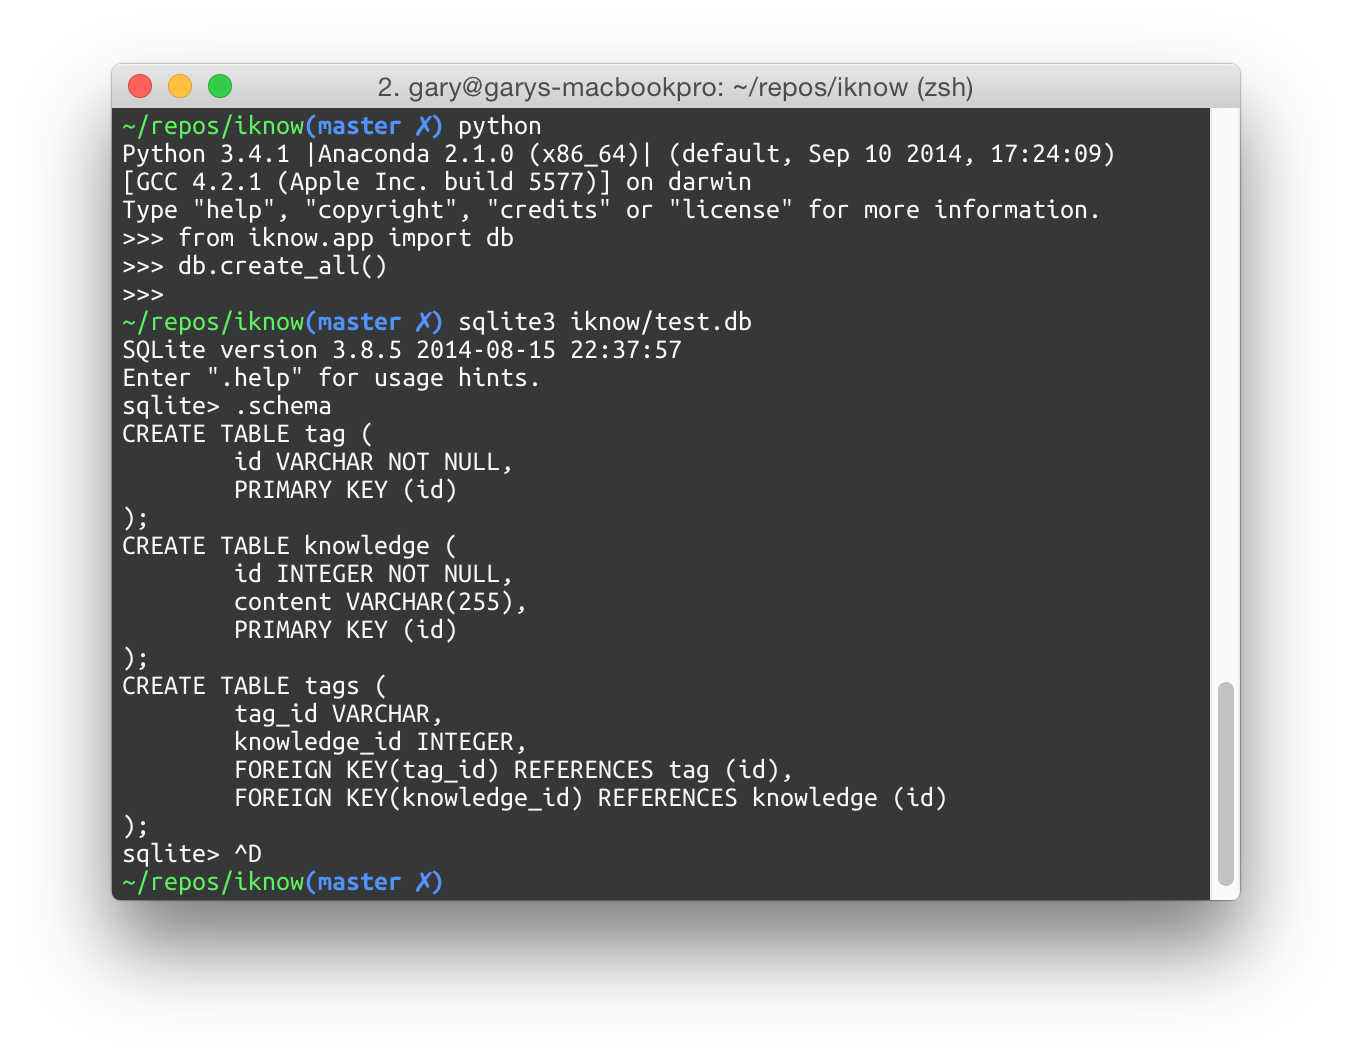
\includegraphics[width=0.7\textwidth]{img/schema}
\end{figure}

\begin{figure}[h!]
  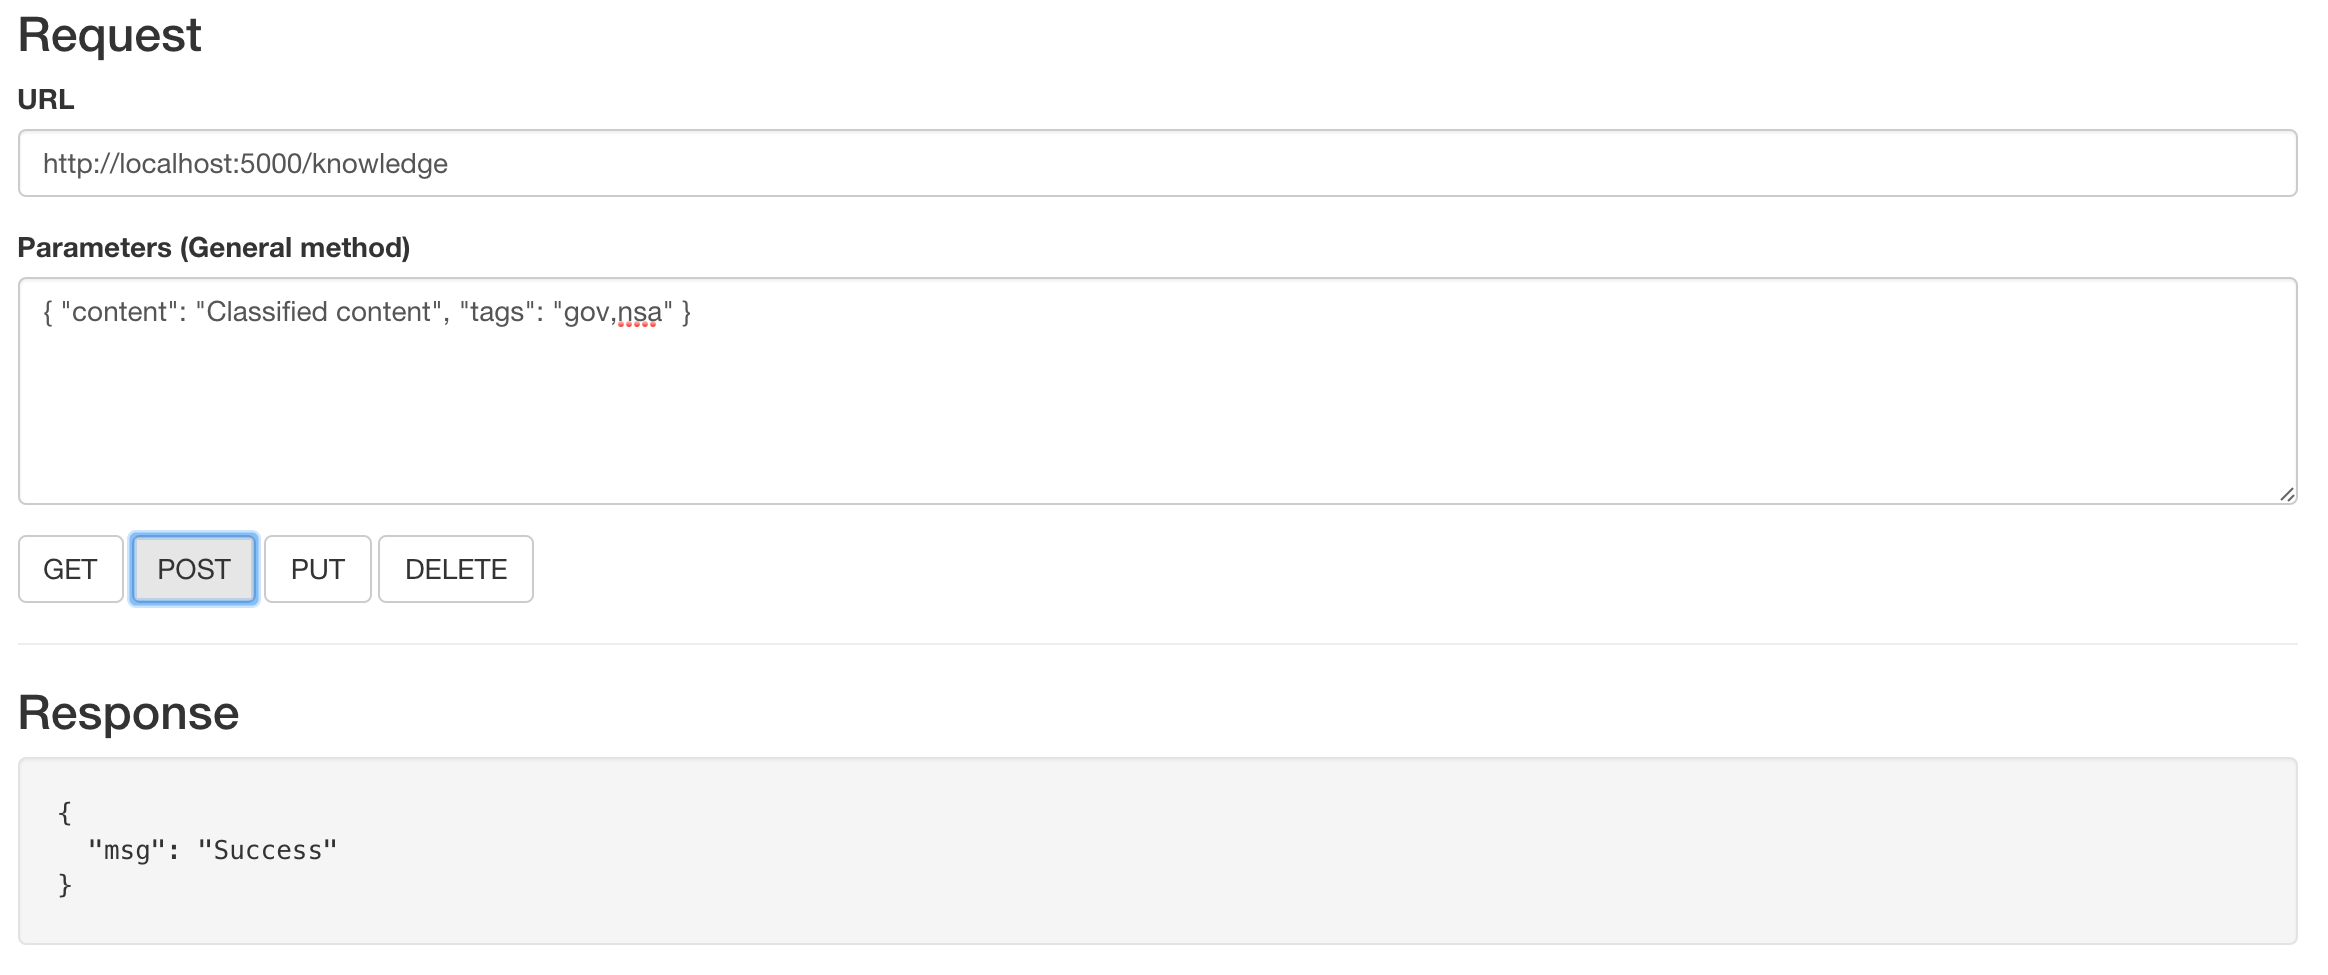
\includegraphics[width=\textwidth]{img/testput0}
\end{figure}

\begin{figure}[h!]
  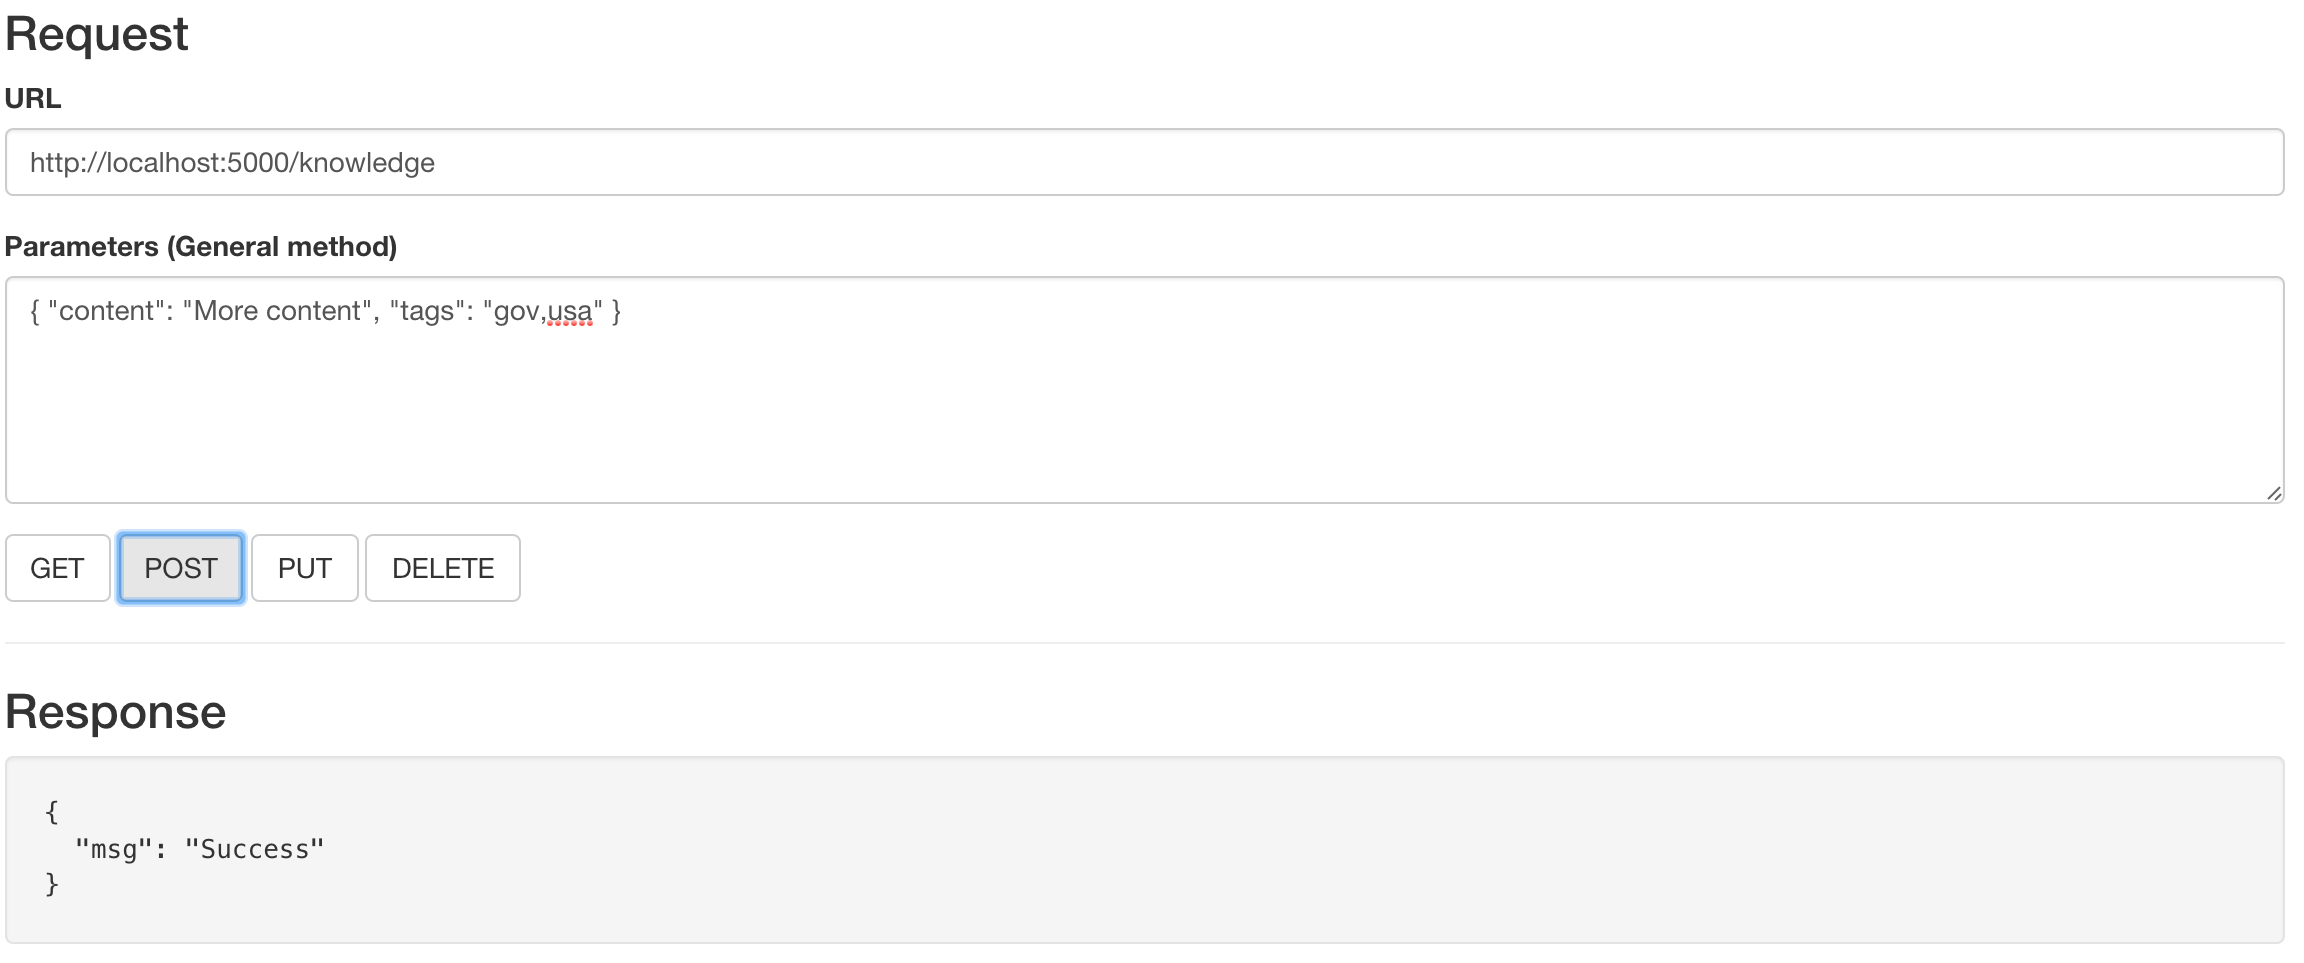
\includegraphics[width=\textwidth]{img/testput1}
\end{figure}



\section{Problems \& Solutions}

\nocite{*}
\bibliographystyle{plain}
\bibliography{bibliography}

\end{document}
